\documentclass[a4paper,10pt]{article}
\input{/home/frr/UFSC/Pagina/Dropbox/Modelos/Modelo_prova_latex/estilo_prova.tex}

\begin{document}


\professor{Fábio Rodrigues de la Rocha}
\turma{06655}
\codigodisciplina{ARA7546}
\disciplina{Circuitos Digitais}
\data{24/03/2014}
\hlimite{20:20}
\listaexercicios{4}

\begin{center}
\large{\fbox{\mbox{Máquinas de Estado}}}
\end{center}

\questao{Construa o circuito de uma máquina de estados do tipo Moore utilizando flip-flops-JK. A máquina em questão deve implementar um contador que conta em
código de gray de 0 até 3 e depois retorna a 0 (saída da máquina). O contador pode funcionar de diferentes modos com base na entrada que pode ser: E1E0= 00 -
contador faz contagem crescente, E1E0=11 - contagem decrescente, E1E0= 01 – contador parado, E1E0=10- contador retorna ao estado 0. Crie a tabela mostrando os
estados, o valor das entradas, os estados futuros, etc. Crie as equações para acionar os flip-flops, crie as equações de saídas, monte o circuito com flip-flops}


\questao{Para acionar um determinado dispositivo eletrônico X é necessário transmitir uma seqüência de valores, um bit por pulso de clock. O dispositivo,
amostra estes valores bit a bit e caso ele detecte que uma seqüência especial (assinatura), o dispositivo será acionado.
Construa uma máquina de estados do tipo Mealy (utilizando flip-flops JK) que reconheça uma seqüência de valores 1011* (Asterisco significa que o valor anterior
pode repetir-se 0 ou mais vezes) ou seja, o dispositivo reconhece os valores 1011, 10111, 101111, etc. Caso a máquina reconheça o valor, sua saída será 1, caso
contrário, será 0. Perceba,  que na seqüência ilustrativa 10101010111 existe uma seqüência que quando lida pela máquina de estados será reconhecida (negrito) e
que quando reconhecida, fará que a máquina tenha saída 1. Perceba ainda, que logo que o valor da seqüência mudar de estado, de forma a descaracterizar a seqüência
especial, a saída fica em 0, como em 10101010111111110.
Apresente o diagrama de estados da máquina de Mealy, construa a tabela de transições de estados e saídas, mostre as equações para J e K de cada um dos flip-flops
(com as simplificações por mapas de Karnaugh) e também a equação da saída da máquina de estados. }


\questao{A figura abaixo mostra um circuito eletrônico resultante de um projeto de uma máquina de estados. Baseado neste, crie as equações de ativação dos FF e
apresente o diagrama de estados. Qual é o tipo de máquina ?}


\begin{figure}[H]
\centering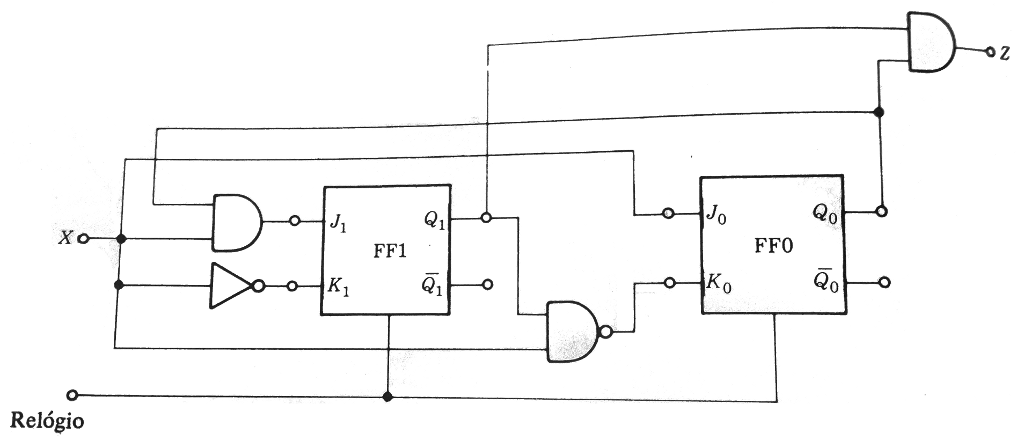
\includegraphics[width=0.6\textwidth]{maquina}

\end{figure}


%\begin{figure}[H]
%\begin{minipage}[b]{0.4\textwidth}
%\centering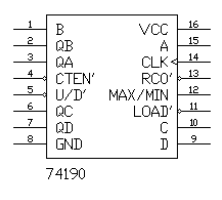
\includegraphics[width=0.6\textwidth]{74190}
%\end{minipage}
%\hspace{0.5cm}
%\begin{minipage}[b]{0.6\textwidth}
%\centering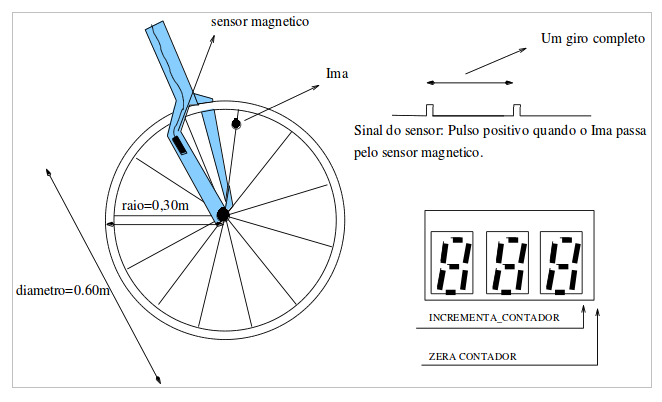
\includegraphics[width=0.6\textwidth]{bicicleta}
%\end{minipage}
%\end{figure}




\end{document}